\documentclass[tikz,border=10pt]{standalone}
% No extra TikZ libraries needed for this figure.
\begin{document}
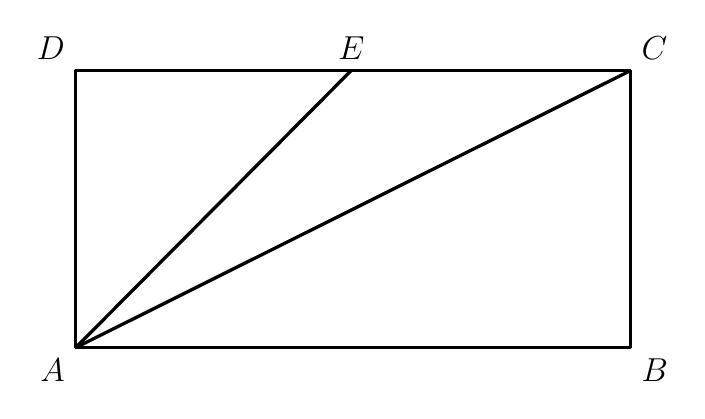
\begin{tikzpicture}[line width=1.2pt, line join=round, font=\fontsize{12}{14.4}\selectfont]

  % Named vertices (scale s = 0.014898 cm/px, A placed at origin, y up)
  \coordinate (A) at (0,0);
  \coordinate (B) at (7.05,0);
  \coordinate (C) at (7.05,3.52);
  \coordinate (D) at (0,3.52);
  \coordinate (E) at (3.50,3.52);

  % Rectangle sides
  \draw (A) -- (B) -- (C) -- (D) -- cycle;

  % Diagonal and segment from A to E
  \draw (A) -- (E);
  \draw (A) -- (C);

  % Vertex labels (math mode)
  \node[below left]  at (A) {$A$};
  \node[below right] at (B) {$B$};
  \node[above right] at (C) {$C$};
  \node[above left]  at (D) {$D$};
  \node[above]       at (E) {$E$};

\end{tikzpicture}
\end{document}